\chapter{Basic Concepts} % (fold)
\label{cha:basic_concepts}

Lorem ipsum dolor sit amet, consectetur adipisicing elit, sed do eiusmod
tempor incididunt ut labore et dolore magna aliqua. Ut enim ad minim veniam,
quis nostrud exercitation ullamco laboris nisi ut aliquip ex ea commodo
consequat. Duis aute irure dolor in reprehenderit in voluptate velit esse
cillum dolore eu fugiat nulla pariatur. Excepteur sint occaecat cupidatat non
proident, sunt in culpa qui officia deserunt mollit anim id est laborum.
%
% * Contextualization
%     * Problems of augmented reality on the web
% * State of the art
%     * History of web ✔
%     * W3C ✔
%     * Browsers ✔
%         * The browser's high level structure ✔
%         * The browser's main functionality ✔
%     * HTML5
%     * JavaScript
%         * Language details ✔
%         * Typed arrays ✔
%         * requestAnimationFrame
%         * getUserMedia
%     * Canvas
%     * Video
%     * WebRTC
%     * APIs
%
\section{Web} % (fold)
\label{sec:basic_concepts:web}

Using concepts from existing hypertext systems, Tim Berners-Lee, computer scientist and at that time employee of CERN, wrote a proposal in March 1989 for what would eventually become the World Wide Web (WWW) \cite{WC2006}.

The World Wide Web is a shared information system operating on top of the Internet. Web browsers retrieve content and display from remote web servers using a stateless and anonymous protocol called HyperText Transfer Protocol (HTTP). Web pages are written using a simple language called HyperText Markup Language (HTML). They may be augmented with other technologies such as Cascading Style Sheets (CSS), which adds additional layout and style information to the page, and JavaScript (JS) language, which allows client-side computation. Browsers typically provide other useful features such as bookmarking, history, password management, and accessibility features to accommodate users with disabilities \cite{Grosskurth2005}.

In the beginning of the web, plain text and images were the most advanced features available on the browsers. In 1994, the World Wide Web Consortium (W3C) was founded to promote interoperability among web technologies. Companies behind web browser development together with the web community, were able to contribute to the W3C specifications \cite{WC2006}. Today's web is a result of the ongoing efforts of an open web community that helps define these technologies and ensure that they're supported in all web browsers. Those contributions transformed the web in a growing universe of interlinked pages and applications, with videos, photos, interactive content, 3D graphics processed by the Graphics Processing Unit (GPU), and other varieties of features without requiring any third-party plugins installation \cite{Hickson2013}. The significant reuse of open source components among different browsers and the emergence of extensive web standards have caused the browsers to exhibit ``convergent evolution'' \cite{Grosskurth2005}.

\subsection{State of the Art} % (fold)
\label{sub:basic_concepts:web:state_of_the_art}

The browser main functionality is to present a web resource, by requesting it from the server and displaying it on the browser window. There are four major browsers used today: Internet Explorer, Firefox, Safari and Chrome. Currently, the usage share of Firefox, Safari and Chrome together is nearly 60\% \cite{Traffic2013}.

Three mature browser implementations were selected and, for each browser, a conceptual architecture was described based on domain knowledge and available documentation. Firefox, Safari and Chrome were used to derive the reference architecture because they are mature systems, have reasonably large developer communities and user bases, provide good support for web standards, and are entirely open source.

The reference architecture for web browsers based on three well known open source implementations architecture, is shown in Figure \ref{figure:web_architecture}; it comprises eight major subsystems plus the dependencies between them: (1) the User Interface, this includes the address bar, back and forward buttons, bookmarking menu \etc\ Every part of the browser display except the main window where you see the requested resource; (2) the Browser Engine, an embeddable component that provides a high-level interface for querying and manipulating the Rendering Engine; (3) the Rendering Engine, which performs parsing and layout for HTML documents, optionally styled with CSS; (4) the Networking subsystem, used for network calls, like HTTP requests. It has platform independent interface and underneath implementations for each platform; (5) the JavaScript Interpreter, used to parse and execute the JavaScript code; (6) the XML Parser; (7) the UI Backend, which provides drawing and windowing primitives, user interface widgets, and fonts. Underneath it uses the operating system user interface methods; and (8) the Data Persistence subsystem, which stores various data associated with the browsing session on disk, including bookmarks, cookies, and cache \cite{Grosskurth2005}.

\begin{figure}[!htb]
  \centering
  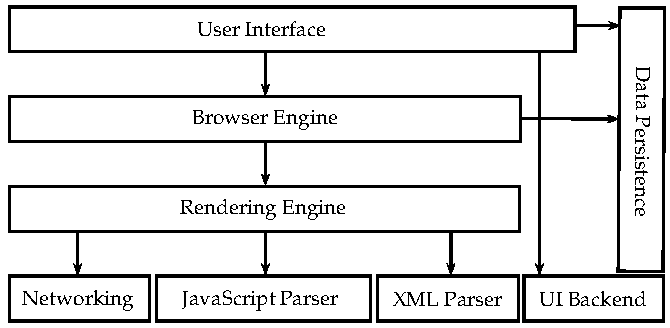
\includegraphics{chapters/basic_concepts/web_architecture.pdf}
  \caption{Reference architecture for web browsers}
  \label{figure:web_architecture}
\end{figure}

Browser subsystem are swappable and could vary for browser vendor, platform or operational system. The browsers mostly differ between different vendors in subsystems (2) the Browser Engine, (3) the Rendering Engine, and (5) the JavaScript Interpreter. Firefox subsystems (2) and (3) is known as Gecko \cite{Firefox2013} \cite{Gecko2013}, Safari as WebKit \cite{Safari2013} \cite{WebKit2013} and Chrome uses a fork of WebKit project called Blink \cite{Chrome2010} \cite{Blink2013}. Those browsers subsystems, often called Browser Engines, are shown on Figure \ref{figure:web_architecture_engines}.

Another common swappable subsystem is (5) the JavaScript Interpreter. JavaScript is a lightweight, interpreted, object-oriented language with first-class functions, most known as the scripting language for Web pages \cite{Gecko2013}. The JavaScript standard is ECMAScript. As of 2013, all modern browsers fully support ECMAScript 5.1. Older browsers support at least ECMAScript 3 \cite{Gecko2013} \cite{International2009}.

\begin{figure}[!htb]
  \centering
  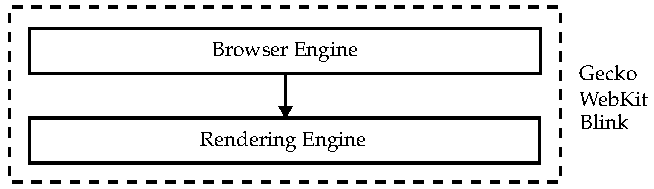
\includegraphics{chapters/basic_concepts/web_architecture_engines.pdf}
  \caption{Reference architecture for browsers engines}
  \label{figure:web_architecture_engines}
\end{figure}

The JavaScript language is intended to be used within some larger environment, be it a browser, server-side scripts, or similar. For a basic example of the language syntax a \textit{println} might have been defined in Listing \ref{lst:javascript_syntax}.

\begin{lstlisting}[label={lst:javascript_syntax},caption=Basic example of JavaScript syntax]
function println(string) {
  window.alert(string);
}
\end{lstlisting}

JavaScript core language features comprises few major features: (1) Functions and function scope, function is a ``subprogram'' that can be called by code external, functions have a scope it references for execution; (2) Global Objects, refer to objects in the global scope, such as general-purpose constructors (\textit{Array, Boolean, Date} \etc), Typed array constructors (\textit{Float32Array, Int32Array, Uint32Array} \etc), Error constructors \etc; (3) Statements, consist of keywords used with the appropriate syntax (\textit{function, if...else, block, break, const, continue, debugger \etc}); (4) Operators and keywords, arithmetic operators ($+, -, *, /,$ \etc), bitwise operators ($\&, |, <<, >>,$ \etc), assignment operators, comparison operators, logical operators, string operators, member operators, conditional operator, \textit{delete} operator, \textit{instanceof} operator, \textit{new} operator, \textit{this} operator, \textit{typeof} operator, \textit{void} operator \etc\ \cite{MDN2013}.

As web applications become more and more powerful, adding features such as audio and video manipulation, access to raw data using WebSockets, and so forth, it has become clear that there are times when it would be helpful for JavaScript code to be able to quickly and easily manipulate raw binary data. In the past, this had to be simulated by treating the raw data as a string and using the \textit{charCodeAt()} method to read the bytes from the data buffer \cite{MDN2013} \cite{TypedArray2013}.

However, this is slow and error-prone, due to the need for multiple conversions, especially if the binary data is not actually byte-format data, but, for example, 32-bit integers or floats.

JavaScript typed arrays provide a mechanism for accessing raw binary data much more efficiently. This thesis takes advantage of typed arrays in order to achieve acceptable performance on the web of complex algorithms implementations.

The three well known open-source browsers, Firefox version 16.0, Safari version 6.0.4 and Chrome version 25.0.1364, were compared in the following benchmark executed on Mac OS X 10.8.3, 2.6 GHz Intel Core i7 16 GB 1600 MHz RAM. The array types selected were \textit{Array}, not strongly typed array; \textit{Float32Array}, represents an array of 32-bit floating point numbers; \textit{Uint8Array}, represents an array of 8-bit unsigned integers. For each array type a read and a write operation was executed $100,000$ times. In order to not compromise benchmark results caused by run-time type conversion \cite{International2009}, the write value used for each array type were proper selected, \eg\ \textit{Number} $1.0$ was used for regular arrays \textit{Array}, \textit{Number} $1.0$ was used for \textit{Float32Array}, and unsigned \textit{Number} $1$ for \textit{Uint8Array}. Regular \textit{vs} typed arrays performance benchmark is shown in Figure \ref{figure:typed_arrays_performance} \cite{TypedArrayPerformance2013}.

As conclusion, typed arrays provides fast read and write operations when compared to regular arrays in JavaScript, \ie\ $7872$ \textit{ops/sec} for unsigned array \textit{vs} $4437$ \textit{ops/sec} in Firefox browser, similar behavior is noticeable on Safari and Chrome, thereby float and unsigned arrays are vastly used on complex algorithms implementations on the web.

\begin{figure}[!htb]
  \begin{tikzpicture}
      \begin{axis}[
          bar width=15pt,
          enlarge x limits=0.25,
          height= 200pt,
          legend cell align=left,
          scaled y ticks=false,
          symbolic x coords={Firefox,Safari,Chrome},
          width=0.85*\textwidth,
          xmajorgrids=true,
          xtick=data,
          ybar=\pgflinewidth,
          ylabel={Operations per second (ops/sec)},
          ylabel style={yshift=10pt},
          ymajorgrids=true,
          ymin=0
      ]
          \addplot[style={wblue, fill=wblue}]
              coordinates {
                (Firefox, 4437)
                (Safari, 2607)
                (Chrome, 679)
              };

          \addplot[style={wred, fill=wred}]
              coordinates {
                (Firefox, 5841)
                (Safari, 2797)
                (Chrome, 1510)
              };

          \addplot[style={worange, fill=worange}]
              coordinates {
                (Firefox, 7872)
                (Safari, 3089)
                (Chrome, 1510)
              };

          \legend{Array,Float32Array,Uint8Array}
      \end{axis}
  \end{tikzpicture}
  \caption{Regular \textit{vs} typed arrays performance benchmark}
  \label{figure:typed_arrays_performance}
\end{figure}

% subsection state_of_the_art (end)

\subsection{Problems of Augmented Reality on the Web} % (fold)
\label{sub:basic_concepts:web:problems_of_augmented_reality_on_the_web}

% subsection problems_of_augmented_reality_on_the_web (end)

% section web (end)

\section{Augmented Reality} % (fold)
\label{sec:basic_concepts:augmented_reality}

Lorem ipsum dolor sit amet, consectetur adipisicing elit, sed do eiusmod
tempor incididunt ut labore et dolore magna aliqua. Ut enim ad minim veniam,
quis nostrud exercitation ullamco laboris nisi ut aliquip ex ea commodo
consequat. Duis aute irure dolor in reprehenderit in voluptate velit esse
cillum dolore eu fugiat nulla pariatur. Excepteur sint occaecat cupidatat non
proident, sunt in culpa qui officia deserunt mollit anim id est laborum.

\subsection{State of the Art} % (fold)
\label{sub:basic_concepts:augmented_reality:state_of_the_art}

Lorem ipsum dolor sit amet, consectetur adipisicing elit, sed do eiusmod
tempor incididunt ut labore et dolore magna aliqua. Ut enim ad minim veniam,
quis nostrud exercitation ullamco laboris nisi ut aliquip ex ea commodo
consequat. Duis aute irure dolor in reprehenderit in voluptate velit esse
cillum dolore eu fugiat nulla pariatur. Excepteur sint occaecat cupidatat non
proident, sunt in culpa qui officia deserunt mollit anim id est laborum.

% subsection state_of_the_art (end)

% section augmented_reality (end)

\section{Tracking and Object Detection} % (fold)
\label{sec:basic_concepts:tracking}

Lorem ipsum dolor sit amet, consectetur adipisicing elit, sed do eiusmod
tempor incididunt ut labore et dolore magna aliqua. Ut enim ad minim veniam,
quis nostrud exercitation ullamco laboris nisi ut aliquip ex ea commodo
consequat. Duis aute irure dolor in reprehenderit in voluptate velit esse
cillum dolore eu fugiat nulla pariatur. Excepteur sint occaecat cupidatat non
proident, sunt in culpa qui officia deserunt mollit anim id est laborum.

\subsection{State of the Art} % (fold)
\label{sub:basic_concepts:tracking:state_of_the_art}

% subsection state_of_the_art (end)

% section tracking (end)

% chapter basic_concepts (end)